\newpage

\section{Desain dan Implementasi}

Tugas ini dilakukan sesuai dengan desain sistem berikut beserta implementasinya. Desain sistem adalah konsep dari pembuatan dan perancangan infrastruktur dan kemudian diwujudkan dalam bentuk alur yang harus dikerjakan


\subsection{Deskripsi sistem}
Pada tugas ini kita akan melakukan analisis data dan membangun model regresi linier untuk memprediksi jumlah penonton video Youtube berdasarkan metadata yang tersedia. Proses ini melibatkan beberapa langkah, mulai dari eksplorasi data hingga evaluasi model. Desain sistem ini mencakup langkah-langkah yang akan dijabarkan dalam Gambar \ref{fig:desain_sistem}.

\begin{figure}[ht]
    \centering
    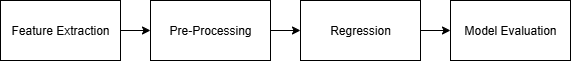
\includegraphics[width=0.8\textwidth]{gambar/metodologi.png}
    \caption{Blok Diagram Sistem}
    \label{fig:desain_sistem}
\end{figure}

\subsection{Feature Extraction}
Feature extraction adalah proses penting dalam machine learning yang bertujuan untuk mengidentifikasi dan memilih fitur-fitur yang relevan dari data yang tersedia. Dalam konteks tugas ini, kita akan melakukan feature extraction pada metadata video Youtube untuk mendapatkan fitur-fitur yang akan digunakan dalam model regresi linier.

\subsubsection{Deskripsi Dataset}
Dataset yang digunakan dalam tugas ini adalah dataset dalam format .xslx yang berisi metadata dari video Youtube. Dataset ini mencakup berbagai informasi seperti judul, deskripsi, tag, kategori, dan statistik penonton. Setiap baris dalam dataset mewakili satu video, dan kolom-kolomnya berisi fitur-fitur yang relevan untuk analisis. Gambar \ref{fig:dataset_youtube} merupakan contoh dari dataset yang digunakan.

\begin{figure}[ht]
    \centering
    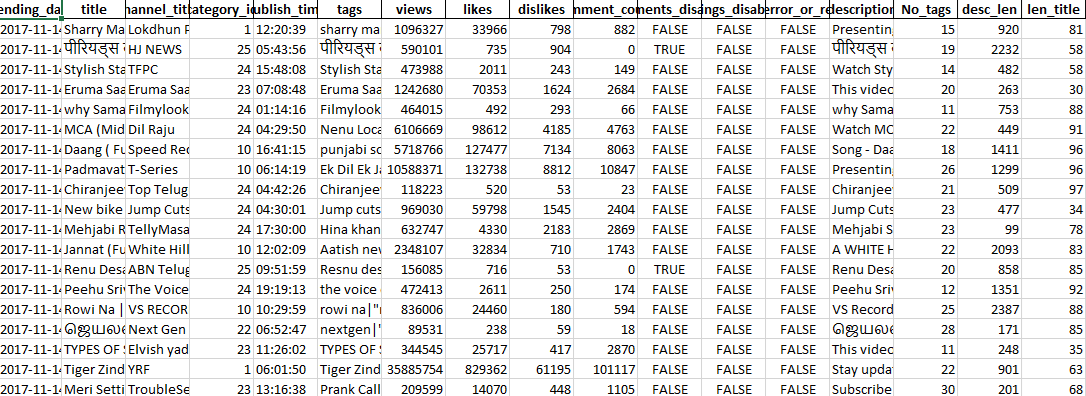
\includegraphics[width=0.6\textwidth]{gambar/dataset.png}
    \caption{Contoh Dataset Youtube}
    \label{fig:dataset_youtube}
\end{figure}
\newpage
Adapun untuk memperjelas fitur-fitur yang digunakan dalam model regresi linier, berikut adalah deskripsi singkat dari beberapa fitur yang terdapat dalam dataset:

\begin{enumerate}
    \item \textbf{trending\_date}: Tanggal ketika video menjadi trending.
    \item \textbf{title}: Judul video.
    \item \textbf{channel\_title}: Nama channel yang mengunggah video.
    \item \textbf{category\_id}: Kategori video dalam label encoding.
    \item \textbf{publish\_time}: Waktu publish video.
    \item \textbf{tags}: Tag yang digunakan pada video.
    \item \textbf{views}: Jumlah views video.
    \item \textbf{likes}: Jumlah likes video.
    \item \textbf{dislikes}: Jumlah dislikes video.
    \item \textbf{comment\_count}: Jumlah komentar pada video.
    \item \textbf{comments\_disabled}: Status apakah komentar dinonaktifkan pada video.
    \item \textbf{ratings\_disabled}: Status apakah rating dinonaktifkan pada video.
    \item \textbf{video\_error\_or\_removed}: Status apakah video error atau sudah dihapus saat ini.
    \item \textbf{description}: Deskripsi video.
    \item \textbf{No\_tags}: Jumlah tag yang digunakan pada video.
    \item \textbf{desc\_len}: Panjang kata deskripsi video.
    \item \textbf{len\_title}: Panjang kata judul video.
    \item \textbf{publish\_date}: Tanggal publish video dalam format datetime.
\end{enumerate}

\subsubsection{EDA (Exploratory Data Analysis)}
Exploratory Data Analysis (EDA) adalah langkah awal yang penting dalam analisis data. EDA membantu kita memahami struktur data, pola, dan hubungan antar fitur sebelum membangun model. Dalam tugas ini, kita akan melakukan EDA pada dataset Youtube untuk mengidentifikasi fitur-fitur yang relevan dan memahami distribusi data.

Dimulai dari statistik deskriptif, kita dapat melihat ringkasan dari setiap fitur dalam dataset. Adapun statistik deskriptif yang dihasilkan dari dataset ini mencakup informasi seperti jumlah data, nilai rata-rata, standar deviasi, nilai minimum, dan nilai maksimum untuk setiap fitur numerik. Statistik deskriptif ini memberikan gambaran awal tentang distribusi data dan membantu dalam mengidentifikasi fitur-fitur yang mungkin memiliki pengaruh signifikan terhadap jumlah penonton video.

Sebelumnya dataset telah diimport ke dalam DataFrame menggunakan pustaka pandas. Dengan mengelompokkan fitur menjadi dua jenis yaitu fitur numerik dan fitur kategorikal, kita dapat melakukan analisis yang lebih terfokus. Fitur numerik mencakup kolom-kolom seperti views, likes, dislikes, comment\_count, No\_tags, desc\_len, dan len\_title. Sedangkan fitur kategorikal mencakup kolom-kolom seperti trending\_date, title, channel\_title, category\_id, publish\_time, tags, comments\_disabled, ratings\_disabled, video\_error\_or\_removed, dan description.

Namun sebelum itu kita perlu melakukan beberapa langkah awal seperti mengimpor library yang diperlukan. Adapun beberapa library tersebut diantaranya adalah pandas, numpy, matplotlib, seaborn, scikit-learn. Library-library ini akan membantu kita dalam melakukan analisis data dan visualisasi.
%verbatim untuk python

\begin{lstlisting}[language=Python, caption=Statistik Deskriptif Fitur Numerik]
import pandas as pd
import seaborn as sns
import matplotlib.pyplot as plt
import numpy as np
\end{lstlisting}

Setelah itu kita dapat memuat dataset ke dalam DataFrame dan melakukan analisis statistik deskriptif. Berikut adalah contoh kode untuk mendapatkan statistik deskriptif dari fitur numerik:

\begin{lstlisting}[language=Python, caption=Statistik Deskriptif Fitur Numerik]
df = pd.read_excel('dataset_youtube.xlsx')

#bagi dataset menjadi fitur numerik dan kategorikal
numerical_features = df.select_dtypes(include=[np.number])
categorical_features = df.select_dtypes(exclude=[np.number])
\end{lstlisting}

Adapun beberapa hal yang harus kita cek terlebih dahulu dalam melakukan analisa agar mendapatkan insight yang baik dalam dataset. Adapun beberapa hal tersebut adalah:

\begin{enumerate}
    \item Cek apakah ada missing value pada dataset.
    \item Cek apakah ada duplikasi data pada dataset.
    \item Cek apakah ada outlier pada fitur numerik.
    \item Cek distribusi dari setiap fitur numerik.
    \item Cek hubungan antar fitur numerik menggunakan heatmap.
\end{enumerate}

Missing value didapatkan dengan mengecek apakah ada nilai yang kosong pada dataframe yang telah diimport. Jika ada, kita dapat menghapus baris yang memiliki missing value atau melakukan imputasi dengan nilai rata-rata atau median dari fitur tersebut. Namun sebelum itu kita perlu mengecek berapa jumlah missing value yang ada pada dataset dan jika jumlahnya sedikit kita dapat menghapusnya.

Dengan menggunakan `isnull()` dan `sum()`, kita dapat melihat jumlah missing value pada setiap kolom. Berikut merupakan outputnya :

\begin{lstlisting}[language=Python, caption=Informasi DataFrame]


title                      0
channel_title              0
category_id                0
publish_time               0
tags                       0
views                      0
likes                      0
dislikes                   0
comment_count              0
comments_disabled          0
ratings_disabled           0
video_error_or_removed     0
description               29
No_tags                    0
desc_len                   0
len_title                  0
publish_date               0
publish_hour               0
publish_period             0
publish_dayofweek          0
is_weekend                 0
dtype: int64

\end{lstlisting}

Disini kita mendapatkan bahwa terdapat missing value pada kolom description sebanyak 29 baris. Kita dapat menghapus baris tersebut karena jumlahnya relatif kecil dibandingkan dengan total data yang ada. Namun kita tidak akan hapus sekarang kita akan hapus setelah semua proses EDA selesai.

Selanjutnya kita cek apakah ada duplikasi data pada dataset. Dalam konteks dataset ini kita tidak akan mengecek duplikasi data berdasarkan seluruh kolom melainkan kita akan cek menggunakan kolom title. Mengapa demikian? karena title adalah kolom yang paling unik dan dapat digunakan sebagai identifikasi video. Kita akan menggunakan fungsi `duplicated()` untuk mengecek apakah ada duplikasi pada kolom title. Berikut adalah contoh output cellnya :



\begin{lstlisting}[language=Python, caption=Cek Duplikasi Data]
    Mission: Impossible - Fallout (2018) - Official Trailer 
    - Paramount Pictures    19

    Name: count, dtype: int64
\end{lstlisting}

Setelah membersihkan data duplikat didapatkan 16431 baris data yang unik. Kita dapat melanjutkan ke langkah berikutnya yaitu mengecek apakah ada outlier pada fitur numerik. Outlier adalah nilai yang jauh berbeda dari nilai lainnya dalam dataset. Outlier dapat mempengaruhi hasil analisis dan model yang dibangun, sehingga penting untuk mengidentifikasinya.

Untuk dapat melihat outlier maka kita dapat menggunakan boxplot. Boxplot adalah visualisasi yang menunjukkan distribusi data dan mengidentifikasi outlier. Kita akan membuat boxplot untuk setiap fitur numerik dalam dataset. Gambar \ref{fig:boxplot_fitur_numerik} merupakan contoh boxplot untuk fitur numerik.

\begin{figure}[ht]
    \centering
    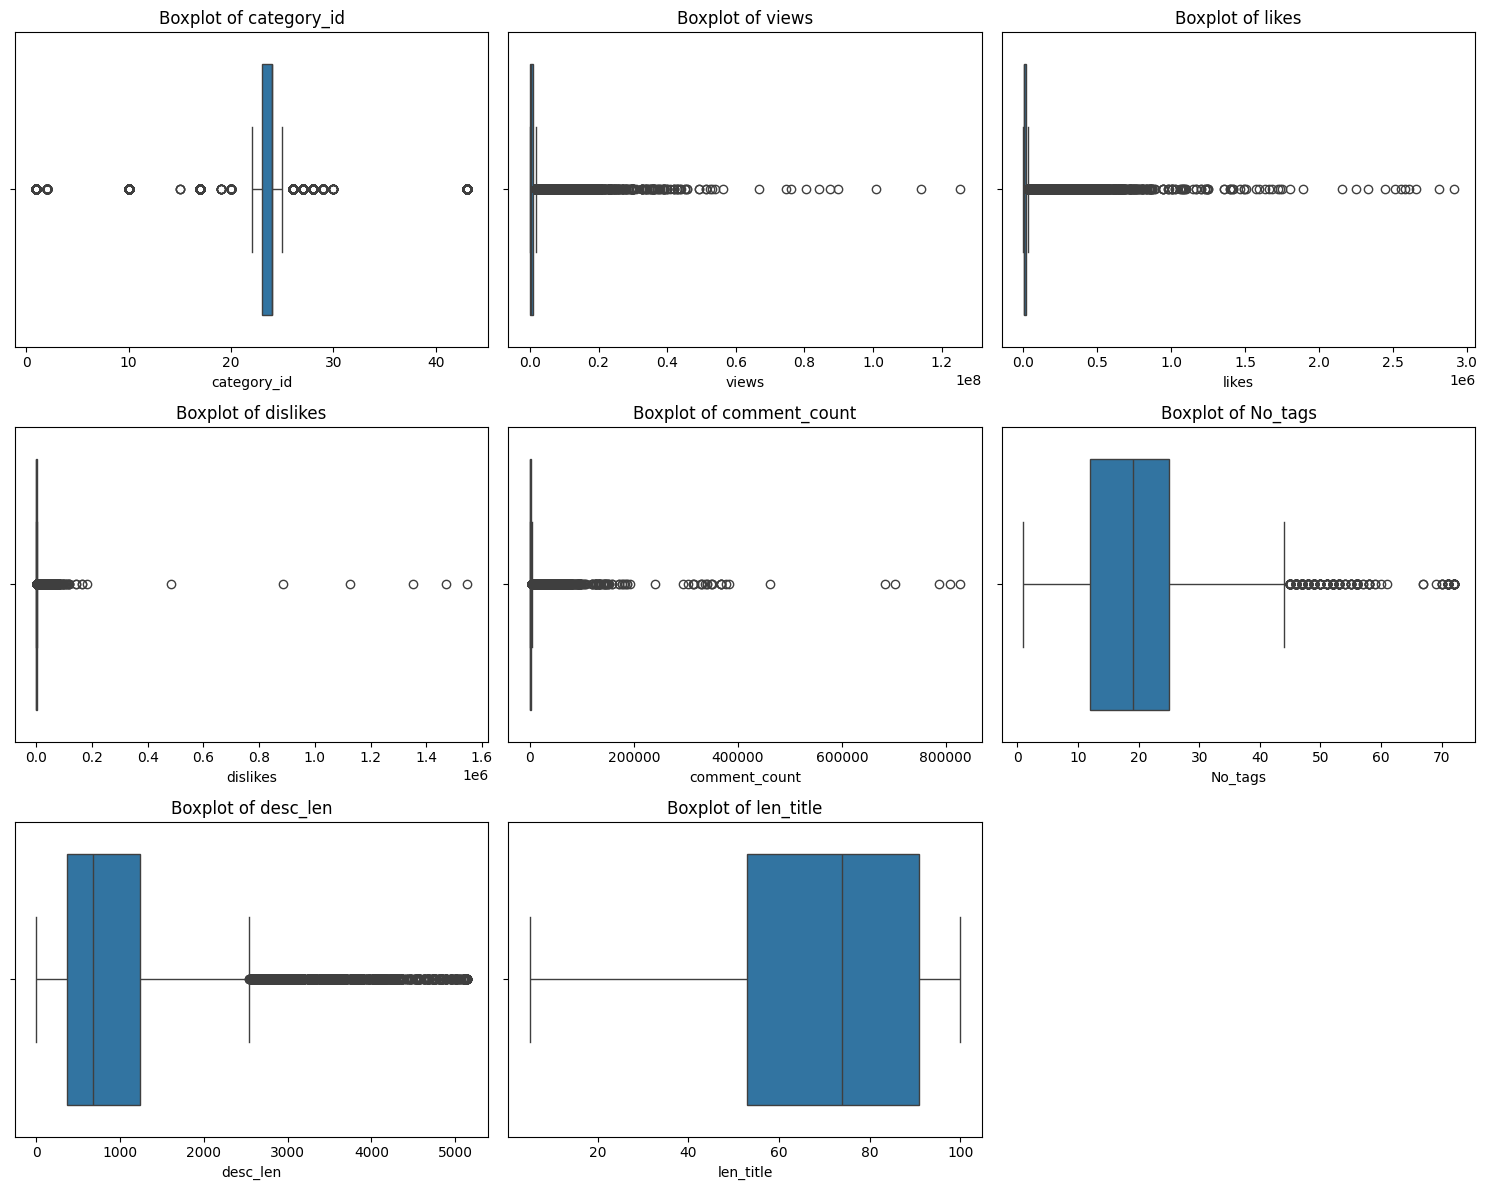
\includegraphics[width=0.8\textwidth]{gambar/boxplot1.png}
    \caption{Boxplot Fitur Numerik}
    \label{fig:boxplot_fitur_numerik}
\end{figure}

Setelah melihat boxplot, kita dapat mengidentifikasi outlier pada fitur numerik dan bagaimana tipe distribusi pada setiap fitur numerik. Kita dapat menghapus outlier tersebut atau melakukan transformasi data untuk mengurangi pengaruhnya terhadap model yang akan dibangun. Berikut merupakan tipe distribusi dari setiap fitur numerik yang ada pada dataset.

\begin{itemize}
    \item \textbf{views}: Distribusi tidak normal, sangat right-skewed.
    \item \textbf{likes}: Distribusi juga right-skewed.
    \item \textbf{dislikes}: Distribusi tidak normal, terdapat outlier yang signifikan.
    \item \textbf{comment\_count}: Distribusi tidak normal, terdapat outlier yang signifikan.
    \item \textbf{No\_tags}: Ada outlier signifikan di atas nilai 50-70.
    \item \textbf{desc\_len}: Ada outlier yang signifikan bahkan lebih banyak dari no\_tags.
    \item \textbf{len\_title}: Distribusi normal, tidak ada outlier yang signifikan walaupun skewed.
\end{itemize}

Selanjutnya kita akan mengecek hubungan antar fitur numerik menggunakan heatmap. Heatmap adalah visualisasi yang menunjukkan korelasi antar fitur numerik dalam dataset. Kita akan menggunakan fungsi `corr()` untuk menghitung korelasi antar fitur numerik dan kemudian membuat heatmap menggunakan seaborn. Gambar \ref{fig:heatmap_fitur_numerik} merupakan heatmap untuk fitur numerik.

\begin{figure}[ht]
    \centering
    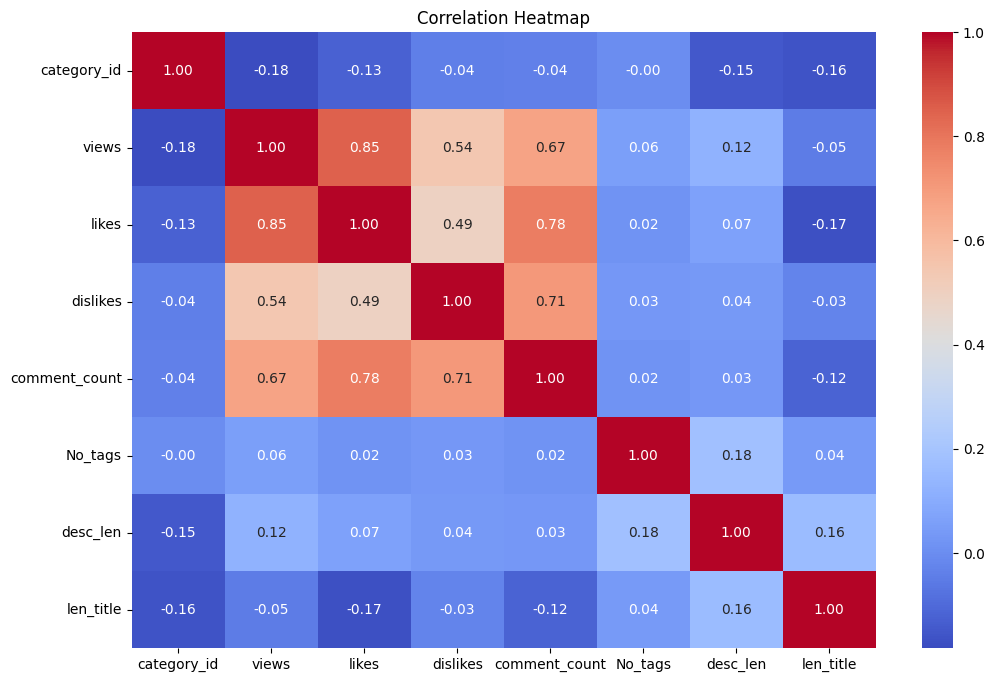
\includegraphics[width=0.8\textwidth]{gambar/heatmap.png}
    \caption{Heatmap Fitur Numerik}
    \label{fig:heatmap_fitur_numerik}
\end{figure}

Berdasarkan visualisasi heatmap korelasi antar fitur numerik, diperoleh beberapa temuan penting sebagai berikut:

\begin{itemize}
    \item \textbf{views} memiliki korelasi sangat kuat dengan \textbf{likes} (\textbf{0.85}) dan korelasi sedang dengan \textbf{comment\_count} (\textbf{0.67}) dan \textbf{dislikes} (\textbf{0.54}). Hal ini menunjukkan bahwa video dengan jumlah penayangan tinggi cenderung juga memiliki banyak likes, komentar, dan dislikes.
    
    \item \textbf{likes} memiliki korelasi tinggi dengan \textbf{comment\_count} (\textbf{0.78}) dan \textbf{dislikes} (\textbf{0.49}). Ini mengindikasikan adanya keterkaitan antara jumlah suka dengan keterlibatan pengguna lainnya.
    
    \item \textbf{dislikes} menunjukkan korelasi sedang dengan \textbf{comment\_count} (\textbf{0.71}), yang bisa diartikan bahwa video dengan banyak komentar cenderung juga memiliki banyak dislike.
    
    \item \textbf{No\_tags}, \textbf{desc\_len}, dan \textbf{len\_title} memiliki korelasi yang sangat rendah dengan fitur-fitur lainnya, termasuk \textbf{views}. Hal ini menunjukkan bahwa jumlah tag, panjang deskripsi, dan panjang judul tidak memiliki hubungan linear yang kuat terhadap keterlibatan pengguna.
    
    \item \textbf{category\_id} menunjukkan korelasi negatif lemah terhadap seluruh fitur, termasuk \textbf{views} (-0.18), \textbf{likes} (-0.13), dan \textbf{len\_title} (-0.16), yang menandakan bahwa kategori video tidak berhubungan kuat secara linier terhadap metrik keterlibatan.
\end{itemize}

Secara umum, fitur-fitur yang memiliki korelasi tinggi satu sama lain dapat menyebabkan multikolinearitas apabila digunakan dalam model regresi linier. Oleh karena itu, perlu dipertimbangkan teknik reduksi fitur atau regularisasi untuk mengurangi dampaknya. Namun kita tahan dulu untuk melakukan reduksi fitur karena kita masih akan melakukan beberapa analisis lagi.

Selanjutnya kita akan cek nilai ukuran pemusatan dan penyebaran dari setiap fitur numerik. Ukuran pemusatan mencakup nilai rata-rata, median, dan modus, sedangkan ukuran penyebaran mencakup rentang, varians, dan deviasi standar. Ukuran-ukuran ini memberikan informasi penting tentang distribusi data dan membantu dalam memahami karakteristik setiap fitur. Gambar \ref{fig:ukuran_pemusatan} merupakan ukuran pemusatan dan penyebaran dari fitur numerik.

\begin{figure}[ht]
    \centering
    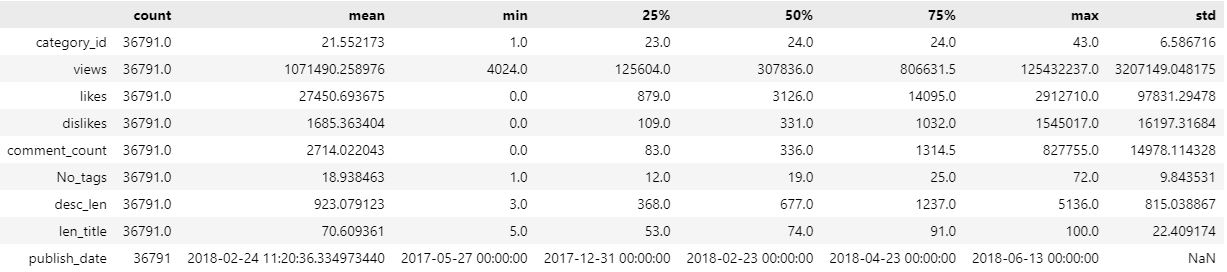
\includegraphics[width=0.8\textwidth]{gambar/pemusatan.png}
    \caption{Ukuran Pemusatan dan Penyebaran Fitur Numerik}
    \label{fig:ukuran_pemusatan}
\end{figure}

Ukuran pemusatan seperti mean, median, dan mode digunakan untuk memberikan gambaran umum mengenai kecenderungan nilai dalam dataset. Meskipun tidak digunakan secara langsung dalam pemodelan, informasi ini bermanfaat dalam tahapan eksplorasi data (EDA). Berikut adalah analisis ringan terhadap fitur numerik pada dataset:

\begin{itemize}
    \item \textbf{views}: Nilai rata-rata (\textit{mean}) sebesar 1.071.490 jauh lebih besar dibandingkan median (307.836) dan modus (105.397), menunjukkan distribusi yang sangat \textit{right-skewed}. Ini mengindikasikan bahwa hanya sebagian kecil video yang memperoleh jumlah tayangan yang sangat tinggi (viral).
    
    \item \textbf{likes}: Rata-rata sebesar 27.450 jauh lebih besar dari median (3.126) dan modus bernilai nol. Ini menunjukkan bahwa banyak video dengan sedikit atau tanpa likes, sementara sebagian kecil lainnya memiliki likes yang sangat tinggi.
    
    \item \textbf{dislikes}: Memiliki rata-rata sebesar 1.685 dan median 331, dengan modus nol. Ini mengindikasikan bahwa sebagian besar video memiliki sedikit atau tidak ada dislike, namun terdapat outlier dengan jumlah dislike yang tinggi.
    
    \item \textbf{comment\_count}: Rata-rata sebesar 2.714 dan median 336, sedangkan modus juga nol. Distribusi yang mirip dengan likes dan dislikes, menunjukkan banyak video yang tidak mendapat komentar.
    
    \item \textbf{category\_id}: Rata-rata sebesar 21,5 dan median 24, dengan modus 24. Karena ini adalah variabel kategori yang direpresentasikan dalam bentuk numerik, ukuran pemusatan tidak terlalu informatif, namun dapat memberi gambaran bahwa kategori dengan ID 24 adalah yang paling dominan dalam dataset.
\end{itemize}

Secara umum, hampir semua fitur numerik memiliki distribusi yang \textit{skewed to the right}, yang merupakan karakteristik umum dalam data platform digital. Ukuran pemusatan ini memperkuat hasil visualisasi yang telah dilakukan sebelumnya.

Ukuran penyebaran menunjukkan seberapa besar variasi atau sebaran nilai dalam data, dan dalam konteks dataset ini, nilai-nilai seperti views, likes, dan comment count memiliki penyebaran yang sangat tinggi, menandakan adanya ketimpangan antara video yang viral dan yang tidak.

Setelah kita menganalisa semuanya kita dapat kesimpulan dari analisis EDA yang telah dilakukan. Berikut adalah ringkasan dari hasil EDA:

\begin{itemize}
    \item Dataset terdiri dari 16431 baris data unik setelah menghapus duplikasi berdasarkan kolom title.
    \item Terdapat missing value pada kolom description sebanyak 29 baris, yang akan dihapus setelah EDA selesai.
    \item Outlier ditemukan pada fitur numerik seperti views, likes, dislikes, comment count, No\_tags, desc\_len, dan len\_title.
    \item Distribusi fitur numerik umumnya tidak normal dan skewed ke kanan.
    \item Korelasi antar fitur numerik menunjukkan hubungan yang signifikan antara views, likes, dan comment count.
    \item Ukuran pemusatan dan penyebaran memberikan gambaran umum tentang distribusi data.
\end{itemize}

\subsection*{Berdasarkan Analisa Lanjutan terhadap Fitur}

Berdasarkan analisis lanjutan terhadap fitur-fitur yang ada, kita dapat menyimpulkan beberapa poin penting:

\begin{itemize}
    \item Fitur-fitur seperti \texttt{likes}, \texttt{dislikes}, dan \texttt{comment\_count} menunjukkan korelasi yang signifikan terhadap variabel target \texttt{views}. Namun, fitur-fitur ini bersifat retrospektif, artinya nilainya hanya tersedia setelah video dipublikasikan dan memperoleh interaksi.
    
    \item Dalam konteks pemodelan prediktif untuk memperkirakan jumlah \texttt{views} pada saat awal publikasi video, fitur-fitur tersebut tidak dapat digunakan karena nilainya belum tersedia (selalu bernilai nol). Oleh karena itu, meskipun secara statistik fitur-fitur ini tampak penting, secara logis dan fungsional tidak relevan untuk dimasukkan dalam model prediksi awal.
    
    \item Sebagai gantinya, fitur-fitur seperti \texttt{publish\_time}, \texttt{category\_id}, dan panjang teks (judul, deskripsi) dipertahankan karena memiliki nilai yang tersedia sebelum publikasi dan dapat berkontribusi terhadap estimasi awal performa video.
    \item Adapun beberapa fitur yang memiliki nilai sangat unik dan tidak relevan seperti \texttt{title}, \texttt{description}, dan \texttt{tags} juga dipertimbangkan untuk dihapus. Meskipun fitur-fitur ini dapat memberikan konteks, mereka tidak memberikan informasi numerik yang dapat digunakan dalam model regresi linier.
\end{itemize}

%#### `Fitur yang di drop`
%Ada beberapa fitur yang harus *dibuang* keputusan ini diambil setelah melakukan analisis menggunakan ilmu peryoutuban, pengukuran statistik, plot, dll. Saya merasa bahwa dengan memasukan like dislikes dan comment_count akan sangat tidak berguna mengingat jika kita ingin memprediksi views apabila kita baru upload video maka like dislike dan comment_count kita pasti 0 dan sangat tidak masuk akal jika kita inputkan nilai 0 tersebut (intinya ga masuk akal), dan untuk trending data juga sama kalau video kita baru upload kan blum trending

%- *likes*
%- *dislikes*
%- *comment_count*
%- *trending_date*

%Saya juga *membuang* fitur yang secara logika tidak penting dan nilainya hampir uniq semua seperti:

%- *title*
%- *description*
%- *tags*
Dari kesimpulan tersebut saya memutuskan untuk membuang fitur-fitur yang tidak relevan dan hanya mempertahankan fitur-fitur yang dapat digunakan untuk memprediksi jumlah views pada saat awal publikasi video. Fitur fitur yang akan saya drop adalah:

\begin{enumerate}
    \item \texttt{likes}
    \item \texttt{dislikes}
    \item \texttt{comment\_count}
    \item \texttt{trending\_date}
    \item \texttt{title}
    \item \texttt{description}
    \item \texttt{tags}
\end{enumerate}

%#### `Fitur yang akan di gunakan`

%Adapun fitur fitur yang akan saya gunakan karena menurut saya lumayan relevan dan mantap.

%- *category_id*
%- *channel_title*
%- *publish_time*
%- *publish_date*

%Fitur yang menurut saya masuk akal juga walaupun saya belum tahu apakah relevan :
%- *No_tags*
%- *desc_len*
%- *len_title*

Selain fitur yang akan saya hapus, adapun fitur fitur yang akan saya gunakan dalam membangun model regresi linier, dimana fitur ini saya anggap relevan dan masuk akal untuk digunakan dalam memprediksi jumlah views pada saat awal publikasi video. Fitur-fitur tersebut adalah:

\begin{enumerate}
    \item \texttt{category\_id}
    \item \texttt{channel\_title}
    \item \texttt{publish\_time}
    \item \texttt{publish\_date}
    \item \texttt{No\_tags}
    \item \texttt{desc\_len}
    \item \texttt{len\_title}
\end{enumerate}

Namun ada beberapa fitur yang semula bernilai timestamp seperti \texttt{publish\_time} dan \texttt{publish\_date} yang akan kita ubah menjadi fitur numerik. Kita akan mengubahnya menjadi fitur numerik dengan cara mengambil informasi dari waktu tersebut seperti hari, jam, dan apakah hari tersebut adalah akhir pekan atau bukan. Hal ini dilakukan agar model regresi linier dapat memahami informasi temporal yang ada pada data.

Adapun saya akan mengubah \texttt{publish\_time} menjadi fitur numerik dengan cara mengambil informasi dari waktu tersebut seperti jam, hari, dan apakah hari tersebut adalah akhir pekan atau bukan. Saya akan membuat beberapa fitur baru sebagai berikut:

\begin{enumerate}
    \item \texttt{publish\_hour}: Jam dari waktu publish video.
    \item \texttt{publish\_dayofweek}: Hari dalam seminggu dari waktu publish video (0-6, dimana 0 adalah Senin).
    \item \texttt{is\_weekend}: Apakah hari tersebut adalah akhir pekan (Sabtu atau Minggu).
    \item \texttt{publish\_period}: Periode waktu publish video (pagi, siang, sore, malam).
\end{enumerate}

Setelah saya ubah maka akan bisa dilakukan encoding baik dari is\_weekend, publish\_period, dan publish\_dayofweek, maupun yang sudah bertipe kategori sebelumnya seperti category\_id, rating\_disabled, dan comments\_disabled. Kita akan melakukan encoding pada fitur-fitur tersebut agar dapat digunakan dalam model regresi linier.

\subsection{Data Preprocessing}
Data preprocessing adalah langkah penting dalam machine learning yang bertujuan untuk mempersiapkan data sebelum digunakan dalam model. Langkah-langkah preprocessing yang akan dilakukan dalam tugas ini akan dijabarkan prosesnya melalui flowchart pada gambar \ref{fig:flowchart_preprocessing}.

\begin{figure}[ht]
    \centering
    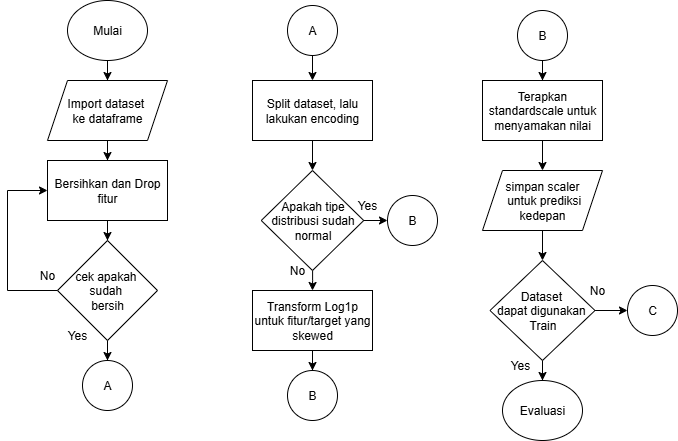
\includegraphics[width=0.6\textwidth]{gambar/flowchart1.png}
    \caption{flowchart preprocessing}
    \label{fig:flowchart_preprocessing}
\end{figure}

Adapun hal pertama yang kita lakukan adalah membersihkan fitur yang tidak relevan seperti yang telah dijelaskan sebelumnya. Kita akan menghapus fitur-fitur yang tidak relevan dan hanya mempertahankan fitur-fitur yang dapat digunakan untuk memprediksi jumlah views pada saat awal publikasi video. Setelah itu kita akan melakukan encoding pada fitur-fitur kategorikal seperti \texttt{category\_id}, \texttt{publish\_dayofweek}, \texttt{is\_weekend}, dan \texttt{publish\_period}.

Kita akan menggunakan teknik one-hot encoding untuk fitur-fitur kategorikal tersebut. One-hot encoding adalah teknik yang mengubah fitur kategorikal menjadi beberapa kolom biner, dimana setiap kolom mewakili satu kategori. Hal ini dilakukan agar model regresi linier dapat memahami informasi dari fitur-fitur kategorikal tersebut. 

Adapun setelah melakukan one hot encoding saya mendapatkan penambahan jumlah fitur sebesar 16 kolom baru yang merupakan hasil dari one hot encoding dari fitur category\_id. Berikut adalah output cellnya:

\begin{figure}[ht]
    \centering
    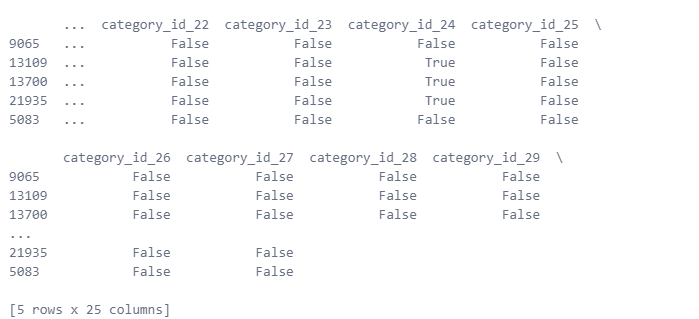
\includegraphics[width=0.8\textwidth]{gambar/onehot.png}
    \caption{One Hot Encoding Fitur Kategorikal}
    \label{fig:one_hot_encoding}
\end{figure}

Selain untuk fitur category\_id saya juga melakukan encoding untuk fitur rating\_disabled, is\_weekend, dan publish\_period. Dengan melakukan encoding pada fitur-fitur tersebut, didapatkan total jumlah fitur sebanyak 24 kolom. 

Setelah itu kita akan melakukan transformasi menggunakan log1p pada fitur-fitur numerik yang akan digunakan. transformasi log1p adalah transformasi yang digunakan untuk mengurangi skewness pada data. Transformasi ini akan mengubah distribusi data menjadi lebih normal dan mengurangi pengaruh outlier terhadap model.

Adapun rumusan dari transformasi log1p adalah sebagai berikut:
\begin{equation}
    \text{log1p}(x) = \log(1 + x)
\end{equation}

Adapun contoh perhitungannya untuk misal 100 views maka akan merubah nilai views tersebut menjadi:

\begin{equation}
    \text{log1p}(100) = \log(1 + 100) = \log(101) \approx 4.615
\end{equation}

\newpage
Dengan melakukan transformasi log1p di tiap baris pada fitur-fitur numerik, kita dapat mengurangi skewness pada data dan membuat distribusi data menjadi lebih normal. Agar lebih jelas, berikut merupakan histogram sebelum dan sesudah transformasi log1p pada label target views :

\begin{figure}[ht]
    \centering
    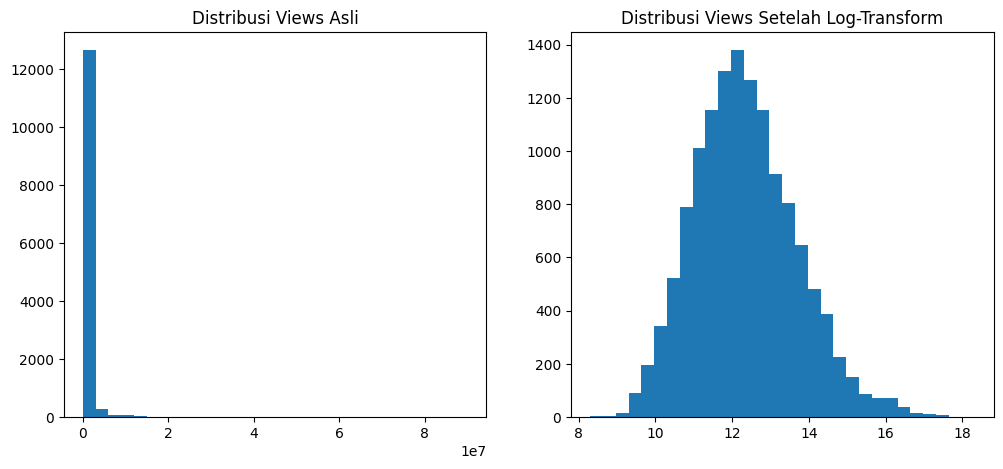
\includegraphics[width=0.8\textwidth]{gambar/logviews.png}
    \caption{Histogram Views Sebelum dan Sesudah Transformasi Log1p}
    \label{fig:histogram_views}
\end{figure}

Namun perlu diingat saat kita melakukan transformasi log1p pada fitur-fitur numerik, kita harus tahu bahwa saat melakukan evaluasi model maka kita harus mengembalikan nilai prediksi ke skala aslinya. Hal ini dilakukan dengan cara melakukan transformasi eksponensial pada nilai prediksi yang dihasilkan oleh model. Transformasi eksponensial adalah kebalikan dari transformasi log1p, sehingga kita dapat mengembalikan nilai prediksi ke skala aslinya.

Adapun rumusan dari transformasi eksponensial adalah sebagai berikut:

%expm1
\begin{equation}
    \text{expm1}(x) = e^x - 1
\end{equation}

Adapun contoh perhitungannya untuk misal 4.615 maka akan merubah nilai views tersebut menjadi:
\begin{equation}
    \text{expm1}(4.615) = e^{4.615} - 1 \approx 100
\end{equation}

Dengan melakukan transformasi eksponensial pada nilai prediksi, kita dapat mengembalikan nilai prediksi ke skala aslinya. Hal ini penting agar kita dapat membandingkan nilai prediksi dengan nilai sebenarnya dari label target views.

Setelah melakukan transformasi biasanya kita akan membuang outlier yang ada pada fitur numerik. Baik menggunakan metode IQR (Interquartile Range) atau Z-score. Namun pada tugas ini kita tidak akan membuang outlier karena kita ingin mempertahankan semua data yang ada. Hal ini dilakukan agar model regresi linier dapat memahami pola-pola yang ada pada data, termasuk pola-pola yang terdapat pada outlier. Mengapa demikian? adapun alasan alasannya sebagai berikut :

%youtube punya viralitas arahkan ke sana
\begin{itemize}
    \item \textbf{Viralitas Video}: Di platform seperti YouTube, video sering kali memiliki potensi untuk menjadi viral. Outlier dalam jumlah views bisa jadi merupakan video yang sangat populer dan memiliki dampak besar. Dengan mempertahankan outlier, model dapat belajar dari pola-pola yang ada pada video-video viral ini.
    
    \item \textbf{Variasi Data}: Outlier sering kali mencerminkan variasi alami dalam data. Menghapusnya dapat menghilangkan informasi penting yang mungkin relevan untuk memahami performa video secara keseluruhan.
    
    \item \textbf{Model Robustness}: Model regresi linier dapat dibuat lebih robust terhadap outlier dengan menggunakan teknik regularisasi seperti Ridge atau Lasso. Ini memungkinkan model untuk tetap belajar dari data meskipun ada beberapa nilai ekstrem, dan model model tersebut juga akan diuji pada tugas ini.
\end{itemize}

Setelah melakukan preprocessing data, kita akan membagi dataset menjadi data latih dan data uji. Pembagian ini penting untuk memastikan bahwa model yang dibangun dapat generalisasi dengan baik pada data yang belum pernah dilihat sebelumnya. Kita akan menggunakan fungsi `train\_test\_split` dari pustaka scikit learn untuk membagi dataset menjadi data latih dan data uji dengan proporsi 80 20.

\begin{lstlisting}[language=Python, caption=Pembagian Data Latih dan Data Uji]

from sklearn.model_selection import train_test_split

# Membagi dataset menjadi data latih dan data uji
X = df.drop(columns=['views'])
y = df['views']

X_train, X_test, y_train, y_test = train_test_split(X, y, test_size
=0.2, random_state=42)
\end{lstlisting}

Dengan pembagian ini, kita akan mendapatkan data latih sebanyak 80\% dari total data dan data uji sebanyak 20\% dari total data. Data latih akan digunakan untuk membangun model regresi linier, sedangkan data uji akan digunakan untuk menguji performa model yang telah dibangun. Adapun shape dari data latih adalah sebagai berikut:

\begin{lstlisting}[language=Python, caption=Shape Data Latih dan uji]

    Shape X_train after scaling: (13144, 26)
    Shape y_train after scaling: (13144,)
    Shape X_test after scaling: (3287, 26)
    Shape y_test after scaling: (3287,)
\end{lstlisting}

Setelah membagi dataset menjadi data latih dan data uji, kita akan melakukan scaling pada fitur-fitur numerik. Scaling adalah langkah penting dalam preprocessing data yang bertujuan untuk mengubah skala fitur-fitur numerik agar memiliki rentang yang sama. Hal ini penting karena model regresi linier sensitif terhadap skala fitur, sehingga scaling dapat membantu meningkatkan performa model.

StandardScaler adalah salah satu teknik scaling yang umum digunakan. Teknik ini akan mengubah fitur-fitur numerik sehingga memiliki rata-rata 0 dan deviasi standar 1. Dengan menggunakan StandardScaler, kita dapat memastikan bahwa semua fitur numerik berada dalam skala yang sama, sehingga model regresi linier dapat belajar dengan lebih baik.

\newpage
Adapun perhitungannya dari StandardScaler adalah sebagai berikut:

\begin{equation}
    z = \frac{x - \mu}{\sigma}
\end{equation}

Dimana:
\begin{itemize}
    \item \( z \) adalah nilai yang telah diskalakan
    \item \( x \) adalah nilai asli dari fitur
    \item \( \mu \) adalah rata-rata dari fitur
    \item \( \sigma \) adalah deviasi standar dari fitur
\end{itemize}

Namun penting untuk menggunakan library joblib untuk menyimpan scaler yang telah dibuat. Hal ini dilakukan agar kita dapat menggunakan scaler yang sama pada data uji saat melakukan prediksi. Dengan menyimpan scaler, kita dapat memastikan bahwa data uji akan diskalakan dengan cara yang sama seperti data latih.

Dengan menerapkan scaler ini maka kita sudah dapat melakukan preprocessing data secara lengkap. Namun kita masih harus drop fitur original dari terutama hasil transform log dan encoding yang tadi sudah kita lakukan. Adapun fitur-fitur yang akan kita drop dapat dilihat pada lstlisting sebagai berikut:

\begin{lstlisting}[language=Python, caption=Drop Fitur Original]

X_train = X_train.drop(['No_tags', 'desc_len'], axis=1)
X_test = X_test.drop(['No_tags', 'desc_len'], axis=1)
X_train = X_train.drop(['publish_time', 'publish_date'], axis=1)
X_test = X_test.drop(['publish_time', 'publish_date'], axis=1)
X_train = X_train.drop(['publish_hour', 'publish_dayofweek', 'is
_weekend', 'publish_period'], axis=1)
\end{lstlisting}
\newpage
Setelah kita drop maka X\_train dan X\_test akan memiliki fitur-fitur yang sudah diproses dan siap digunakan untuk membangun model regresi linier. Gambar \ref{fig:input_data} merupakan gambar input data yang telah diproses.

\begin{figure}[ht]
    \centering
    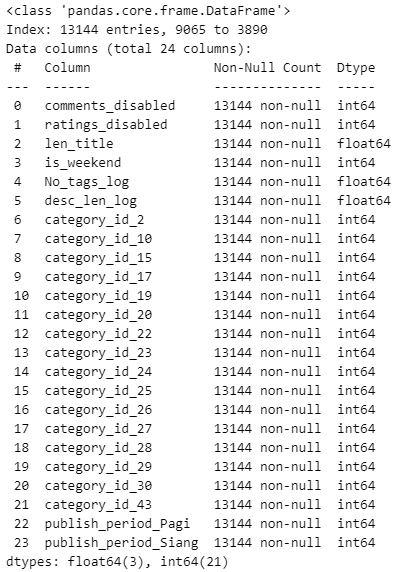
\includegraphics[width=0.4\textwidth]{gambar/input_data.png}
    \caption{Input Data Setelah Preprocessing}
    \label{fig:input_data}
\end{figure}

Setelah melakukan preprocessing data, kita akan mendapatkan data latih dan data uji yang siap digunakan untuk membangun model regresi linier. Data latih akan digunakan untuk melatih model, sedangkan data uji akan digunakan untuk menguji performa model yang telah dibangun. Dengan demikian, kita telah menyelesaikan tahap preprocessing data dalam tugas ini.